\documentclass{homework}

\usepackage{tcolorbox}
\usepackage{etoolbox}
\usepackage{svg}
\usepackage{algorithm}
\usepackage{algpseudocode}
\usepackage{caption}
\usepackage[newfloat]{minted}
\usepackage{pgfplots}
\usepackage{tabularx}
\pgfplotsset{width=10cm,compat=1.9}
\usepackage[super]{nth}
\usepackage{awesomebox}
\usepackage{environ}
\usepackage{tikz}
\usetikzlibrary{shapes, arrows}
\usetikzlibrary{fit,backgrounds,calc}
\usepackage{dirtree}
\usepackage[linguistics]{forest}
\usepackage[showframe]{geometry}

\makeatletter                                       
\newenvironment{chapquote}[3][2.7em]
  {\setlength{\@tempdima}{#1}
   \ifx\relax#2\relax\setlength{\@tempdimb}{#1}\else\setlength{\@tempdimb}{#2}\fi
   \def\chapquote@author{#3}
   \parshape 1 \@tempdima \dimexpr\textwidth-\@tempdima-\@tempdimb\relax
   \itshape}
  {\newline\par\normalfont\hfill--\ \chapquote@author\hspace*{\@tempdimb}\par\bigskip}
\makeatother
\begin{document}
\title{Cloud Computing HW 1 - Simple Web Server}
\author{32190984 Isu Kim}
\maketitle

\newminted{python}{frame=lines,framerule=2pt}
\newenvironment{code}{\captionsetup{type=listing}}{}
\SetupFloatingEnvironment{listing}{name=Code Snippet}

\tikzstyle{startstop} = [rectangle, rounded corners, minimum width=3cm, minimum height=1cm,text centered, draw=black, fill=red!30]
\tikzstyle{process} = [rectangle, minimum width=3cm, minimum height=1cm, text centered, draw=black, fill=orange!30]
\tikzstyle{io} = [trapezium, trapezium left angle=70, trapezium right angle=110, minimum width=3cm, minimum height=1cm, text centered, draw=black, fill=blue!30]
\tikzstyle{arrow} = [thick,->,>=stealth]

\maketitle
\pagebreak

\section{Index}
\begin{enumerate}
   \item Index
   \item Introduction
   \item Design \& Implementation
   \item User Guide \& Demonstration
   \item Evaluation \& Conclusion
\end{enumerate}
 
\section{Introduction}
The main goal of this assignment was to implement a simple web server that runs an HTTP server. However, the assignment has a restriction not to use high-level HTTP API frameworks (e.g. \texttt{Flask} \texttt{NodeJS}), but rather stick to the original socket programming instead. 

In this document, we introduce a simple web server named \texttt{engineX}. \texttt{engineX} supports following features:

\begin{itemize}
    \item \textbf{Multi-clients}: Multiple clients can access the web server concurrently
    \item \textbf{Basic HTTP Operations}: Supports standard \texttt{GET}, \texttt{POST}, \texttt{UPDATE} and \texttt{DELETE}.
    \item \textbf{Dynamic Contents}: Supports \texttt{HTML} and \texttt{text} content parsing.
    \item \textbf{HTTP Response Codes}: Returns ISO HTTP response code.
\end{itemize}

\texttt{engineX} was implemented with C language and was confirmed to work with multiple scenarios under Ubuntu 22.04 environment. The full source code can be found at \href{https://github.com/isu-kim/kloud-computing-dku/tree/main/hw1}{https://github.com/isu-kim/kloud-computing-dku/tree/main/hw1}.

In section 3, the document will deal with simple design and implementation for \texttt{engineX}. In section 4, the user guide and actual demonstrations of the software will be introduced. Finally, in section 5, we will be discussing about performance numbers and methods to improve performance as well as the conclusion.

\section{Design \& Implementation}
\subsection{Multi-Threading}
The most important consideration of \texttt{engineX} is that it should support multiple concurrent clients at once. Meaning that the software must support multi-threading or multi-processing. \texttt{engineX} utilizes multi-threading instead of multi-processing. The main reason for this is the performance overhead of the forking process. It is a well-known fact that forking a new child process usually demands more computing resource compared to creating a simple thread (i.e. lightweight process). 

The following figure describes a sequence of system calls involved in basic socket programming. In our case, this will be an HTTP client connecting to \texttt{engineX}.

\pagebreak
\begin{figure}[h]
\begin{center}
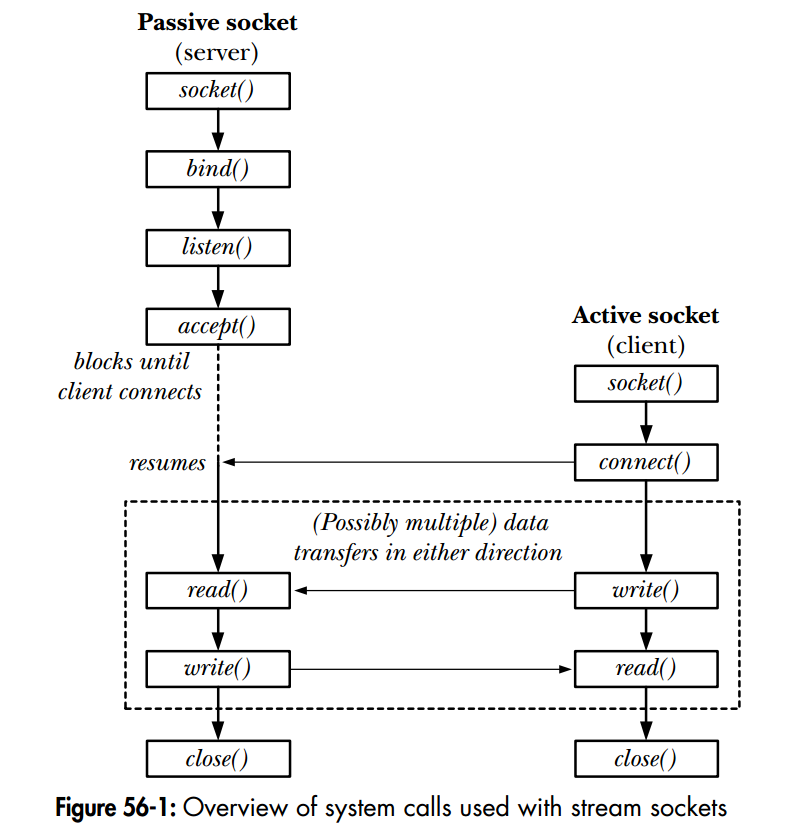
\includegraphics[scale=0.35]{1_socket_flow.png}    
\caption{Socket Workflow}
\end{center}
\end{figure}

For us to achieve multiple clients at once, each client connection should be processed in a separate worker thread. As Figure 2 shows, once a new connection has been established from a HTTP client, the sequences after \texttt{accept} which is \texttt{recv} and \texttt{write} should be processed by a worker thread. 

\begin{figure}[h]
\begin{center}
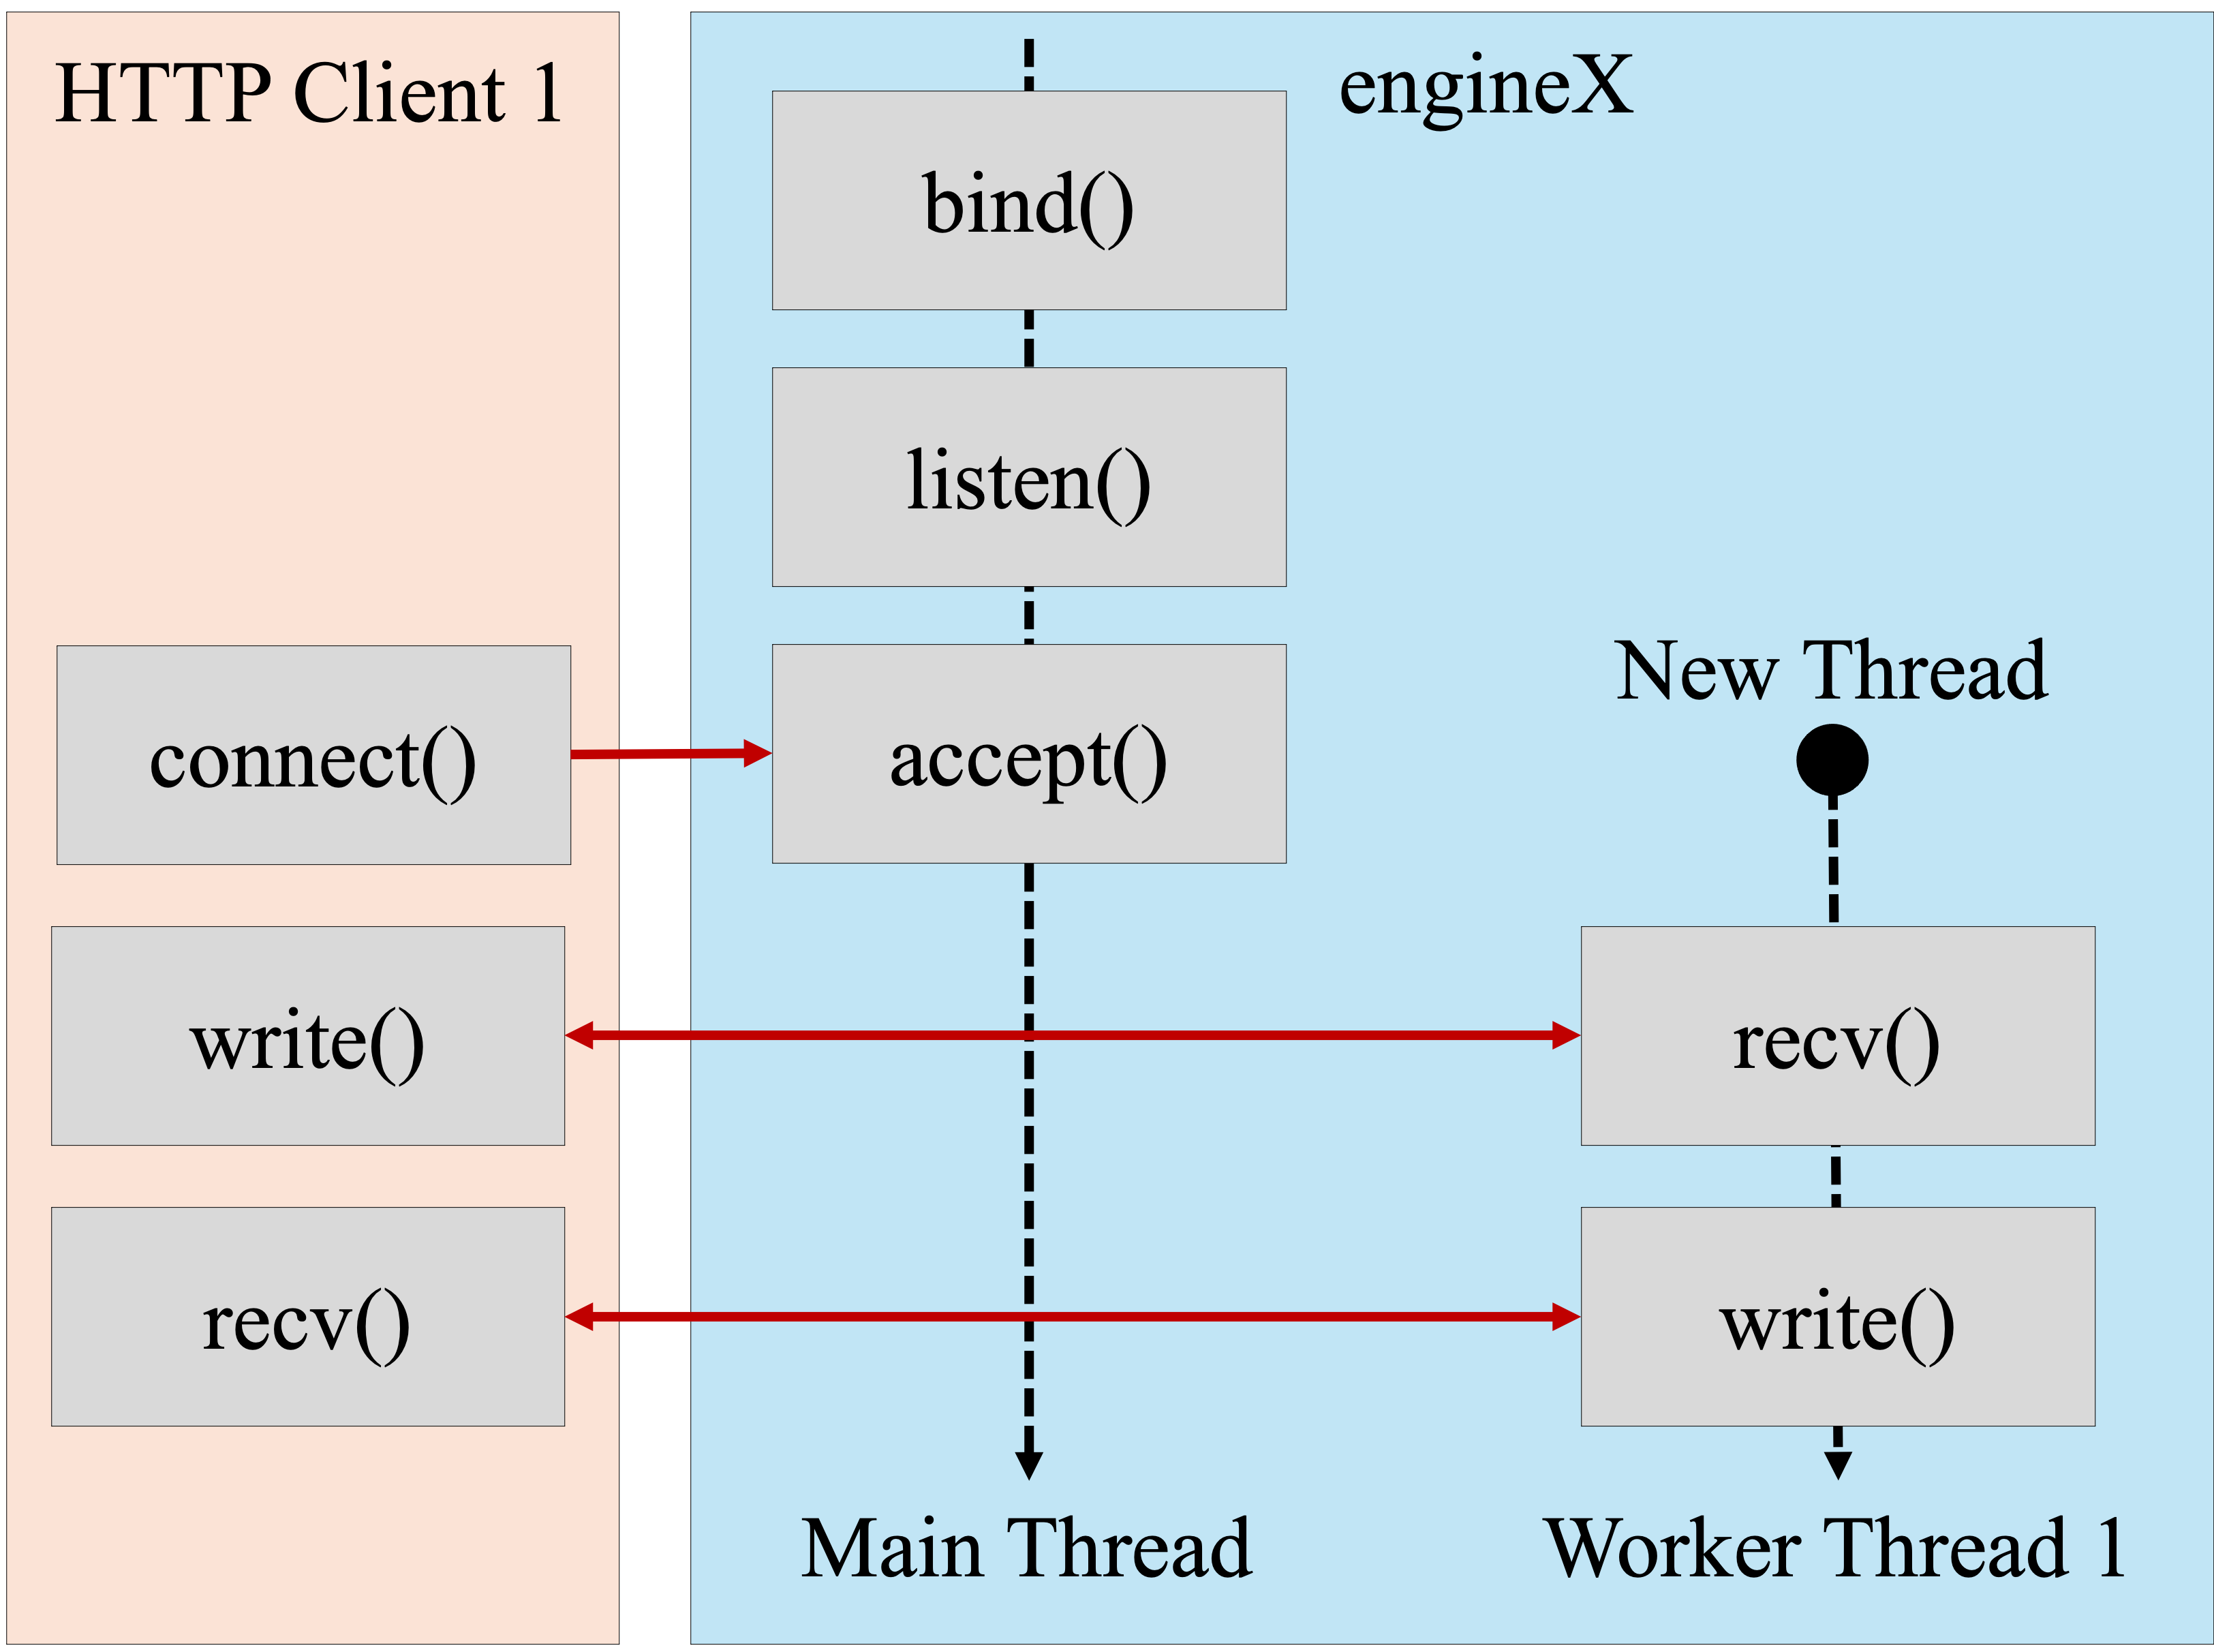
\includegraphics[scale=0.30]{2_single_client.png}    
\caption{Single Client Workflow}
\end{center}
\end{figure}

Once another HTTP client arrives, the new client will be assigned to a new worker thread. The web server is not involved in that much of a race conditions. Each thread will just take care of one remote HTTP client, therefore there will be almost no synchronization required. 

There might be some cases when aclient is performing \texttt{POST} or \texttt{UPDATE} request and another client is performing \texttt{GET} request, which can potentially be a problem. However, this can be easily solved by using OS tricks such as locking files, and this is can be considered as an out of scope since \texttt{engineX} is mainly aimed to provide simple web server.
\pagebreak

\subsection{Workflow}
The following Figure 3 shows a simplified behavior of \texttt{engineX} for a new connection.

\begin{figure}[h]
\begin{center}
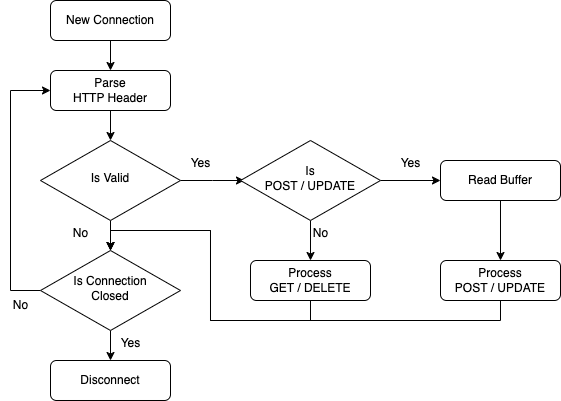
\includegraphics[scale=0.6]{3_flow_chart.png}    
\caption{Connection Flow Chart}
\end{center}
\end{figure}

\subsubsection{Parsing HTTP Header}
Once a new connection is established, the server will first read the buffer using \texttt{read}. Then it will try to parse the basic HTTP header. In this step, the server will look for the following elements:

\begin{itemize}
    \item \textbf{Method}: The HTTP request method. Currently supports \texttt{GET}, \texttt{POST}, \texttt{UPDATE}, \texttt{DELETE}.
    \item \textbf{Endpoint}: The URI that contains the file's name.
    \item \textbf{HTTP Version}: The string that contains the HTTP version such as \texttt{HTTP/1.1}
\end{itemize}

This was implemented using the basic C library's string utilities (i.e. \texttt{string.h}). There might be some cases when the client yet did not send the request information, in that case the server will try to read the buffer again unless the connection is closed.

\subsubsection{Processing Request}
Once the program has determined the method of the HTTP request, the server will now check if the request was \texttt{POST} or \texttt{UPDATE}. For those two cases, the client will send files. Therefore, the server needs to read the buffer with the content size provided in the HTTP header to receive the payloads. Once the payload is read, the server will create a new file or update an existing file using the payload received.

If the request was \texttt{GET} or \texttt{DELETE}, which does not require additional payloads, the server will immediately retrieve or delete the designated file.

All requests will be performed and the results will be sent back to the client using HTTP response. If the user's request was successfully performed, this will return 200. The current HTTP response codes that were implemented are as it follows:


\begin{itemize}
    \item \texttt{200 OK}: User request was successfully performed
    \item \texttt{403 Forbidden}: The user did not have enough permission. This will be triggered when the designated file was not able to be read or modified by \texttt{engineX} process.
    \item \texttt{404 Not Found}: The file was not found under web directory.
    \item \texttt{413 Content Too Large}: The payload exceeds the maximum request payload content size. This is set as 4MB by default.
    \item \texttt{503 Internal Server Error}: \texttt{engineX} was unable to perform request. 
\end{itemize}

If the request failed, the server will return the reason why the request failed. This will be returned as a string that represents the reason for \texttt{errno} defined in Linux.

\subsubsection{Checking Connection}
Once the server returns the response back to the HTTP client, the client might have closed the connection or kept the connection open for the next request. Therefore, the server checks if the socket connection is opened or not.

If the connection was identified as closed, the thread that is taking care of this connection will terminate. If not, the thread will keep servicing the requests.
\pagebreak

\section{User Guide \& Demonstration}
\subsection{Environment}
The environment that this program was checked running is as it follows:
\begin{itemize}
    \item \textbf{OS}: Ubuntu 22.04.01 LTS \textbf{Little Endian}
    \item \textbf{CPU}: Intel(R) Core(TM) i9-7940X CPU @ 3.10GHz
    \item \textbf{RAM}: 64GB
    \item \textbf{Compiler}: GCC 11.3.0, Make 4.3
    \item \textbf{C}: C99
\end{itemize}

\subsection{Building \texttt{engineX}}
\texttt{engineX} offers \texttt{Makefile}, it provides following recipes:
\begin{enumerate}
    \item \texttt{clean}: Cleans up the whole build, this also cleans up the web directory.
    \item \texttt{build}: Builds \texttt{engineX}.
    \item \texttt{debug}: Builds \texttt{engineX} in debug mode. This version of \texttt{engineX} will provide extra information on how the program is running.
\end{enumerate}

For the end-user case, it is suggested to use \texttt{build}. An example terminal output can be like below:
\\
\begin{center}
\begin{code}
\begin{minted}[frame=single,framesep=10pt]{c}
$ git clone https://github.com/isu-kim/kloud-computing-dku.git
$ cd kloud-computing-dku/hw1/
$ make build
make engineX
gcc -O2 -Wall -std=gnu99 -c main.c -o main.o
gcc -O2 -Wall -std=gnu99 -c common/context.c -o common/context.o
gcc -O2 -Wall -std=gnu99 -c common/messages.c -o common/messages.o
gcc -O2 -Wall -std=gnu99 -c http/server.c -o http/server.o
...
gcc -o engineX main.o common/context.o ...
\end{minted}
\captionof{listing}{Example Output of Building \texttt{engineX}}
\end{code}
\end{center}

This will create an executable named \texttt{engineX}. \texttt{engineX} also provides command-line interfaces to run the software. The list shows available choices:

\begin{itemize}
    \item \texttt{--help}, \texttt{-h}: Print out help message.
    \item \texttt{--port}, \texttt{-p}: Specify an port to listen HTTP server, defaults to \texttt{5000}.
    \item \texttt{--listen}, \texttt{-l}: Specify an IPv4 address to listen HTTP server, defaults to \texttt{0.0.0.0}.
    \item \texttt{--files}, \texttt{-f}: Specify directory of web files, defaults to \texttt{web/}.
\end{itemize}

An example execution command will be as follows:
\\
\begin{center}
\begin{code}
\begin{minted}[frame=single,framesep=10pt]{c}
$./engineX --port 8123 --listen 0.0.0.0       
...
engineX - Simple Web Server by isu-kim (https://github.com/isu-kim/)
[2024-04-14 21:16:16] [INFO] Initializing commandline arguments
[2024-04-14 21:16:16] [INFO] No web files directory was specified, using ...
[2024-04-14 21:16:16] [INFO] Initialized arguments
- port=8123
- listen=0.0.0.0
- files_directory=web/
[2024-04-14 21:16:16] [INFO] Starting server...
[2024-04-14 21:16:16] [INFO] Checking web files directory
[2024-04-14 21:16:16] [INFO] Web files directory does not exist, creating one...
[2024-04-14 21:16:16] [INFO] Listening on 0.0.0.0:8123
\end{minted}
\captionof{listing}{Example Output of Executing \texttt{engineX}}
\end{code}
\end{center}

This will start up the web server in \texttt{0.0.0.0:8123}. The web server's file directory will be designated to \texttt{web/}. \texttt{engineX} provides default endpoint which is \texttt{/}. You can use your browser to check the server is up and running. Figure 4 demonstrates an example screenshot of visiting the website using Chrome browser.

\begin{figure}[h]
\begin{center}
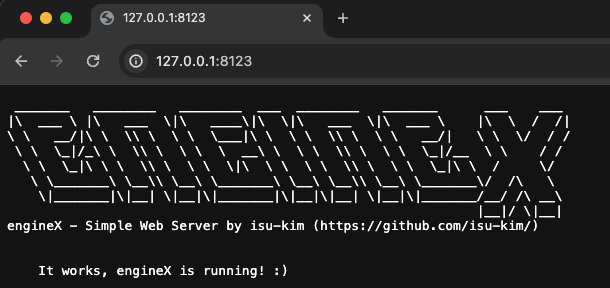
\includegraphics[scale=0.6]{4_ss1.png}    
\caption{Screenshot of Web Browser}
\end{center}
\end{figure}

Meanwhile, you can check the website is running using commands such as \texttt{curl}.
\\
\begin{center}
\begin{code}
\begin{minted}[frame=single,framesep=10pt]{c}
$ curl http://127.0.0.1:8123
...
engineX - Simple Web Server by isu-kim (https://github.com/isu-kim/)


    It works, engineX is running! :)        
\end{minted}
\captionof{listing}{Example Output of Executing \texttt{curl}}
\end{code}
\end{center}
\pagebreak

\subsection{POST Method}
\texttt{engineX} supports \texttt{POST} request which sends a text file to server. This will create the file under the designated endpoint. An example command is as follows:
\\
\begin{center}
\begin{code}
\begin{minted}[frame=single,framesep=10pt]{c}
$ curl -X POST --upload-file "isu.html" http://127.0.0.1:8123/isu.html
Successfully written file as web//isu.html: 232 bytes
\end{minted}
\captionof{listing}{Example Output of \texttt{POST} using \texttt{curl}}
\end{code}
\end{center}

This will \texttt{POST} the file \texttt{isu.html} in the local directory as endpoint \texttt{isu.html}. In the server, the log will show that the request has been successfully processed like below:
\\
\begin{center}
\begin{code}
\begin{minted}[frame=single,framesep=10pt]{c}
... [INFO] [Worker][127.0.0.1:17104] Successfully written file web//isu.html
... [INFO] [Worker][127.0.0.1:17104][200] POST /isu.html HTTP/1.1
\end{minted}
\captionof{listing}{Example Output of \texttt{engineX} after \texttt{POST}}
\end{code}
\end{center}

Also, in the \texttt{web} directory, there will be a new file \texttt{isu.html}.
\\
\begin{center}
\begin{code}
\begin{minted}[frame=single,framesep=10pt]{c}
$ ls web/
isu.html
\end{minted}
\captionof{listing}{Example Output of \texttt{POST} Result}
\end{code}
\end{center}

\warningbox{
    \begin{itemize}
        \item The maximum file size is defined as 2MB. If you wish to post larger file than 2MB, modify the size defined as \texttt{HTTP_MAX_REQUEST_LEN} in \texttt{common/defines.h}
        \item \texttt{POST} method only supports text files. Posting binary files or using form-based requests might not work. Meaning that the \texttt{curl -X POST --upload-file "path/to/your/file.txt"} was tested only.
        \item \texttt{POST} method only supports creating new files. If you would like to change the file contents, use \texttt{UPDATE}.
    \end{itemize}
}

\pagebreak
\subsection{GET Method}
Figure 5 shows the screenshot that that the HTML file uploaded in 4.3 was rendered.

\begin{figure}[h]
\begin{center}
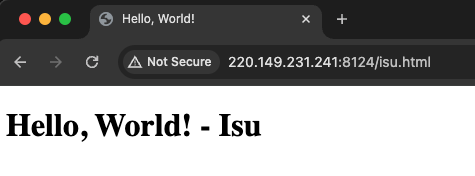
\includegraphics[scale=0.6]{5_ss2.png}    
\caption{Screenshot of Web Browser}
\end{center}
\end{figure}

Now, if we change the permission of \texttt{web/isu.html} to a value that is not accessible by \texttt{engineX} process, the following page will be shown.

\begin{figure}[h]
\begin{center}
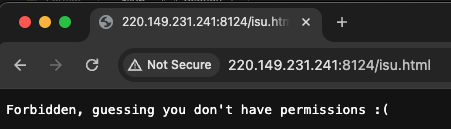
\includegraphics[scale=0.6]{6_ss3.png}    
\caption{Screenshot of Web Browser}
\end{center}
\end{figure}

This will show that the user did not have enough permission to read the file. Also, the response code will come as 403 forbidden. Once we delete the file, the page will show that there is no such file like the following figure.

\begin{figure}[h]
\begin{center}
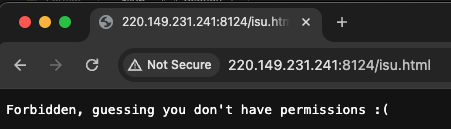
\includegraphics[scale=0.6]{6_ss3.png}    
\caption{Screenshot of Web Browser}
\end{center}
\end{figure}

\warningbox{
\begin{itemize}
    \item The server will serve its type as \texttt{text/text} or \texttt{text/html} according to the file's extension. If the file ends with \texttt{.html}, the file will be served as \texttt{text/html}. Other content types were not defined.
    \item The server can only serve contents up to 4MB. You can adjust this value by modifying \texttt{HTTP_MAX_RESPONSE_LEN} under \texttt{common/defines.h}.
\end{itemize}
    
}

\pagebreak
\subsection{UPDATE Method}
\texttt{engineX} supports \texttt{UPDATE} method, which can overwrite the content of an existing file. This only works if the file already exists. An example command is as follows:
\\
\begin{center}
\begin{code}
\begin{minted}[frame=single,framesep=10pt]{c}
$ curl -X UPDATE --upload-file "isu-mod.html" http://127.0.0.1:8124/isu.html
Successfully updated file web//isu.html 232->267 bytes
\end{minted}
\captionof{listing}{Example Output of \texttt{UPDATE} using \texttt{curl}}
\end{code}
\end{center}
This will upload the file \texttt{isu-mod.html} in the local directory and overwrite the content of \texttt{web/isu.html}. Meanwhile, in the server, the log will show that the request has been successfully processed like below:
\\
\begin{center}
\begin{code}
\begin{minted}[frame=single,framesep=10pt]{c}
... [INFO] [Worker][127.0.0.1:45225] Successfully written file web//isu.html
... [INFO] [Worker][127.0.0.1:45225][200] UPDATE /isu.html HTTP/1.1
\end{minted}
\captionof{listing}{Example Output of \texttt{engineX} after \texttt{UPDATE}}
\end{code}
\end{center}

As we have updated the file, you can see the changes in using the browser. As compared to Figure 5, Figure 8 demonstrates that the web page has changed. 

\begin{figure}[h]
\begin{center}
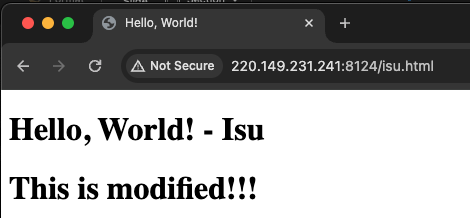
\includegraphics[scale=0.6]{8_ss5.png}    
\caption{Screenshot of Web Browser}
\end{center}
\end{figure}

\warningbox{
    \begin{itemize}
        \item The maximum file size is defined as 2MB. If you wish to upload larger file than 2MB, modify the size defined as \texttt{HTTP_MAX_REQUEST_LEN} in \texttt{common/defines.h}
        \item \texttt{UPDATE} method only supports text files. Posting binary files or using form-based requests might not work. Meaning that the \texttt{curl -X UPDATE --upload-file "path/to/your/file.txt"} was tested only.
    \end{itemize}
}
\pagebreak

\subsection{DELETE Method}
\texttt{engineX} supports \texttt{DELETE} method. This deletes an existing file. An example command is as below:
\\
\begin{center}
\begin{code}
\begin{minted}[frame=single,framesep=10pt]{c}
$ curl -X DELETE http://127.0.0.1:8124/isu.html
Successfully deleted file web//isu.html
\end{minted}
\captionof{listing}{Example Output of \texttt{engineX} after \texttt{DELETE}}
\end{code}
\end{center}

This will delete the file \texttt{web/isu.html}. Meanwhile, in the server, the log will show that the request has been successfully processed like below:
\\
\begin{center}
\begin{code}
\begin{minted}[frame=single,framesep=10pt]{c}
... [INFO] [Worker][127.0.0.1:3308][200] DELETE /isu.html HTTP/1.1
\end{minted}
\captionof{listing}{Example Output of \texttt{engineX} after \texttt{UPDATE}}
\end{code}
\end{center}

Since the file was deleted, the endpoint will no longer be able to be accessed. The following figure shows that the server returns 404 not found.

\begin{figure}[h]
\begin{center}

\includegraphics[scale=0.6]{9_ss6.png}    
\caption{Screenshot of Web Browser}
\end{center}
\end{figure}

\pagebreak

\section{Evaluation \& Conclusion}
\subsection{Evaluation}
To check the performance of \texttt{engineX}, I have used \texttt{wrk} to generate workload and query a single endpoint. For the experiment, the \texttt{wrk} was running with 32 threads with 32 connections for 5 seconds. In order to minimize the parameters affecting the performance, the benchmark was executed in the same machine as \texttt{engineX}. This will avoid inaccuracy caused by network IO to an extent. An example output was as it follows:
\\
\begin{center}
\begin{code}
\begin{minted}[frame=single,framesep=10pt]{c}
$ wrk -t32 -c32 -d5s http://127.0.0.1:8124
Running 5s test http://127.0.0.1:8124
 32 threads and 32 connections
 Thread Stats  Avg   Stdev   Max  +/- Stdev
  Latency   2.98ms  4.12ms 48.04ms  83.45%
  Req/Sec  329.43  631.35   2.97k  93.69%
 14562 requests in 5.10s, 10.50MB read
 Non-2xx or 3xx responses: 1
Requests/sec:  2855.06
Transfer/sec:   2.06MB
\end{minted}
\captionof{listing}{Example Output of \texttt{wrk}}
\end{code}
\end{center}

The output shows that \texttt{engineX} is capable of serving 2855 requests with only one failure. In order to compare with production-grade application, I have tested the same parameters with Nginx. Nginx was set to have only one worker process. The results were as follows:
\\
\begin{figure}[h]
\begin{center}
\begin{tabular}{|l|l|l|}
    \hline
        \textbf{Type} & \textbf{Nginx} & \textbf{engineX} \\
    \hline
        \texttt{Requests/sec} & 21684 & 2855 \\
        \texttt{Transfer/sec(MB)} & 17.76 & 2.06 \\
    \hline
\end{tabular}
\caption{Table of Performance against Nginx}
\end{center}
\end{figure}
\\
The table shows that we have failed to beat Nginx. The performance was around 1/10 of the performance that Nginx offers. To improve \texttt{engineX} in the future, I have investigated potential bottlenecks as well as performance overheads that might have occurred. The following content shows the processes where the performance impact was considered to be high.

\subsubsection{Receiving Packets}
Currently, the server relies on \texttt{read} function which regularly checks if the client has sent a packet to the server. However, since this is done as an infinite loop, the server is running as if it is doing a busy waiting. This will require more resource usage. Therefore, to solve this issue, using \texttt{epoll} or \texttt{select} on the socket file descriptor and triggering the events once a TCP packet has arrived would be a better choice.

\subsubsection{Single Request per Connection}
Currently, each worker thread can only take care of a single request at once. The current implementation only processes a single received packet at once. In order to maximize concurrency, each worker thread that are dealing with a single connection shall be able to create another child thread that takes care of read and write operations. This is the main reason why \texttt{engineX} is struggling with performance issues.

\subsubsection{HTTP Header Parsing}
The current implementation of parsing HTTP headers heavily relies on string operations, which are highly considered a bottleneck. For example, \texttt{engineX} uses \texttt{strstr} or \texttt{strcmp} functions from \texttt{string.h} which are normally a high overhead due to its high time complexity. Therefore, optimizing string parsing part will be better choice in the future.

\subsubsection{Heap Memory Issues}
The current implementation of responding packets requires allocating and deallocating heap memory. Since the response body itself is around 4MB, utilizing heap memory instead of function's stack memory s required. However, since heap memory allocation takes more time, there is a potential performance drop.

\subsubsection{No Caching Involved}
The current implementation does not have any caching methods. If \texttt{engineX} performs caching for \texttt{GET} requests, this will avoid reading the file over and over again for a same content.

\subsection{Conclusion}
Implementing \texttt{engineX} was a lot of fun. However, the worst part was dealing with strings in C using \texttt{string.h}. Since C language utilizes string as \texttt{char[]}, this was especially difficult to be processed properly. Since offsets of strings and size of strings matter, there were lots of segmentation faults as well as buffer overflows. 

Meanwhile, implementing socket network programming was a lot of fun. Since I was familiar with using HTTP or REST API frameworks such as \texttt{Flask}, \texttt{Gin} from \texttt{python} or \texttt{golang}, building \texttt{engineX} from scratch was a lot of fun. Also, it was interesting to see the contents served from my server was actually being rendered in the browser properly as if they were served by other web servers. Also, for performance optimization, I have looked up for \texttt{epoll} and \texttt{select} which can trigger TCP packet arrivals for higher performance and this was a nice experience.

In summary, this was a nice assignment to see how sockets and they act in the lower level. In the future, I would like to optimize the performance up to 50\% of the performance that Nginx offers.

\end{document}
